\documentclass{beamer}
\usepackage[utf8]{inputenc}
\usepackage[T1]{fontenc}
\usepackage{tikz, calc, amsmath, mathtools, hyperref}
\usepackage{graphicx}
\graphicspath{{figures/}}
\usepackage{caption}
\usepackage{bm}
\usepackage[italian]{babel}
\renewcommand{\v}[1]{\boldsymbol{#1}}
%%%%%%%%%%%%%%%%%%%%%%%%%%%%%%%%%%%%%%%%%%%%%%%%%
%  Set Up Manuale della prima maledetta pagina  %
%%%%%%%%%%%%%%%%%%%%%%%%%%%%%%%%%%%%%%%%%%%%%%%%%
\makeatletter % Fare alla lettera???
\setbeamertemplate{title page}{%
  \vskip2em\par
  \vbox{}% Questi due fanno spazio 
  \vfill%  verticale 
  \begingroup
    \centering
    % ColorBox di Title e Subtitle
    \begin{beamercolorbox}[sep=8pt,center]{title}
      \usebeamerfont{title}\inserttitle\par%
      \ifx\insertsubtitle\@empty%
      \else%
        \vskip0.25em%
        {\usebeamerfont{subtitle}\usebeamercolor[fg]{subtitle}\insertsubtitle\par}%
      \fi%     
    \end{beamercolorbox}%
%
    \vskip2em\par

    % Logo Università
    \begin{figure}
	
\includegraphics[width=1.5cm]{figures/Unipi.png}
    \end{figure}
%
    \vskip1em\par
    \vfill%<- added

    % Autore
    \begin{beamercolorbox}[sep=8pt,center]{author}
      \usebeamerfont{author}\insertauthor
    \end{beamercolorbox}
    \vfill%<- added
%
    % Istituto
    \begin{beamercolorbox}[sep=8pt,center]{institute}
      \usebeamerfont{institute}\insertinstitute
    \end{beamercolorbox}
    \vfill%<- added
%
    % Data
    \begin{beamercolorbox}[sep=8pt,center]{date}
      \usebeamerfont{date}\insertdate
    \end{beamercolorbox}%
    \vskip0cm%<- changed
%    {\usebeamercolor[fg]{titlegraphic}\inserttitlegraphic\par}
  \endgroup
%  \vfill%<- removed
}
\makeatother

% Sfondo personalizzato
% \setbeamertemplate{background}{
%     \begin{tikzpicture}
% 	\node[opacity=0.35] {\includegraphics[height=\paperheight,width=\paperwidth]{../Figure/Lorenz1.png}};
%     \end{tikzpicture}
% }
% 
\setbeamerfont{title}{size=\Huge}
\setbeamerfont{author}{size=\Large}

\renewcommand{\v}[1]{\boldsymbol{#1}}



\newcommand{\incfig}[1]{%
    \def\svgwidth{\columnwidth}
    \import{./figures/}{#1.pdf_tex}
}

\title{Caos nel sistema di Lotka-Volterra Competitivo}
\subtitle[SisComp]{Dinamica Non Lineare}
\date[]{}
\author[Edoardo Gabrielli]{Edoardo Gabrielli}
\institute[Unipi]{Università di Pisa}
\usetheme{Singapore}

\AtBeginSection[]
{
    \begin{frame}
	\begin{center}
        \tableofcontents[currentsection]
	\end{center}
    \end{frame}
}

\begin{document}
{% Aggiungo sfondo al titolo
\usebackgroundtemplate{
    \begin{tikzpicture}
	\node[opacity=0.8] 
	    {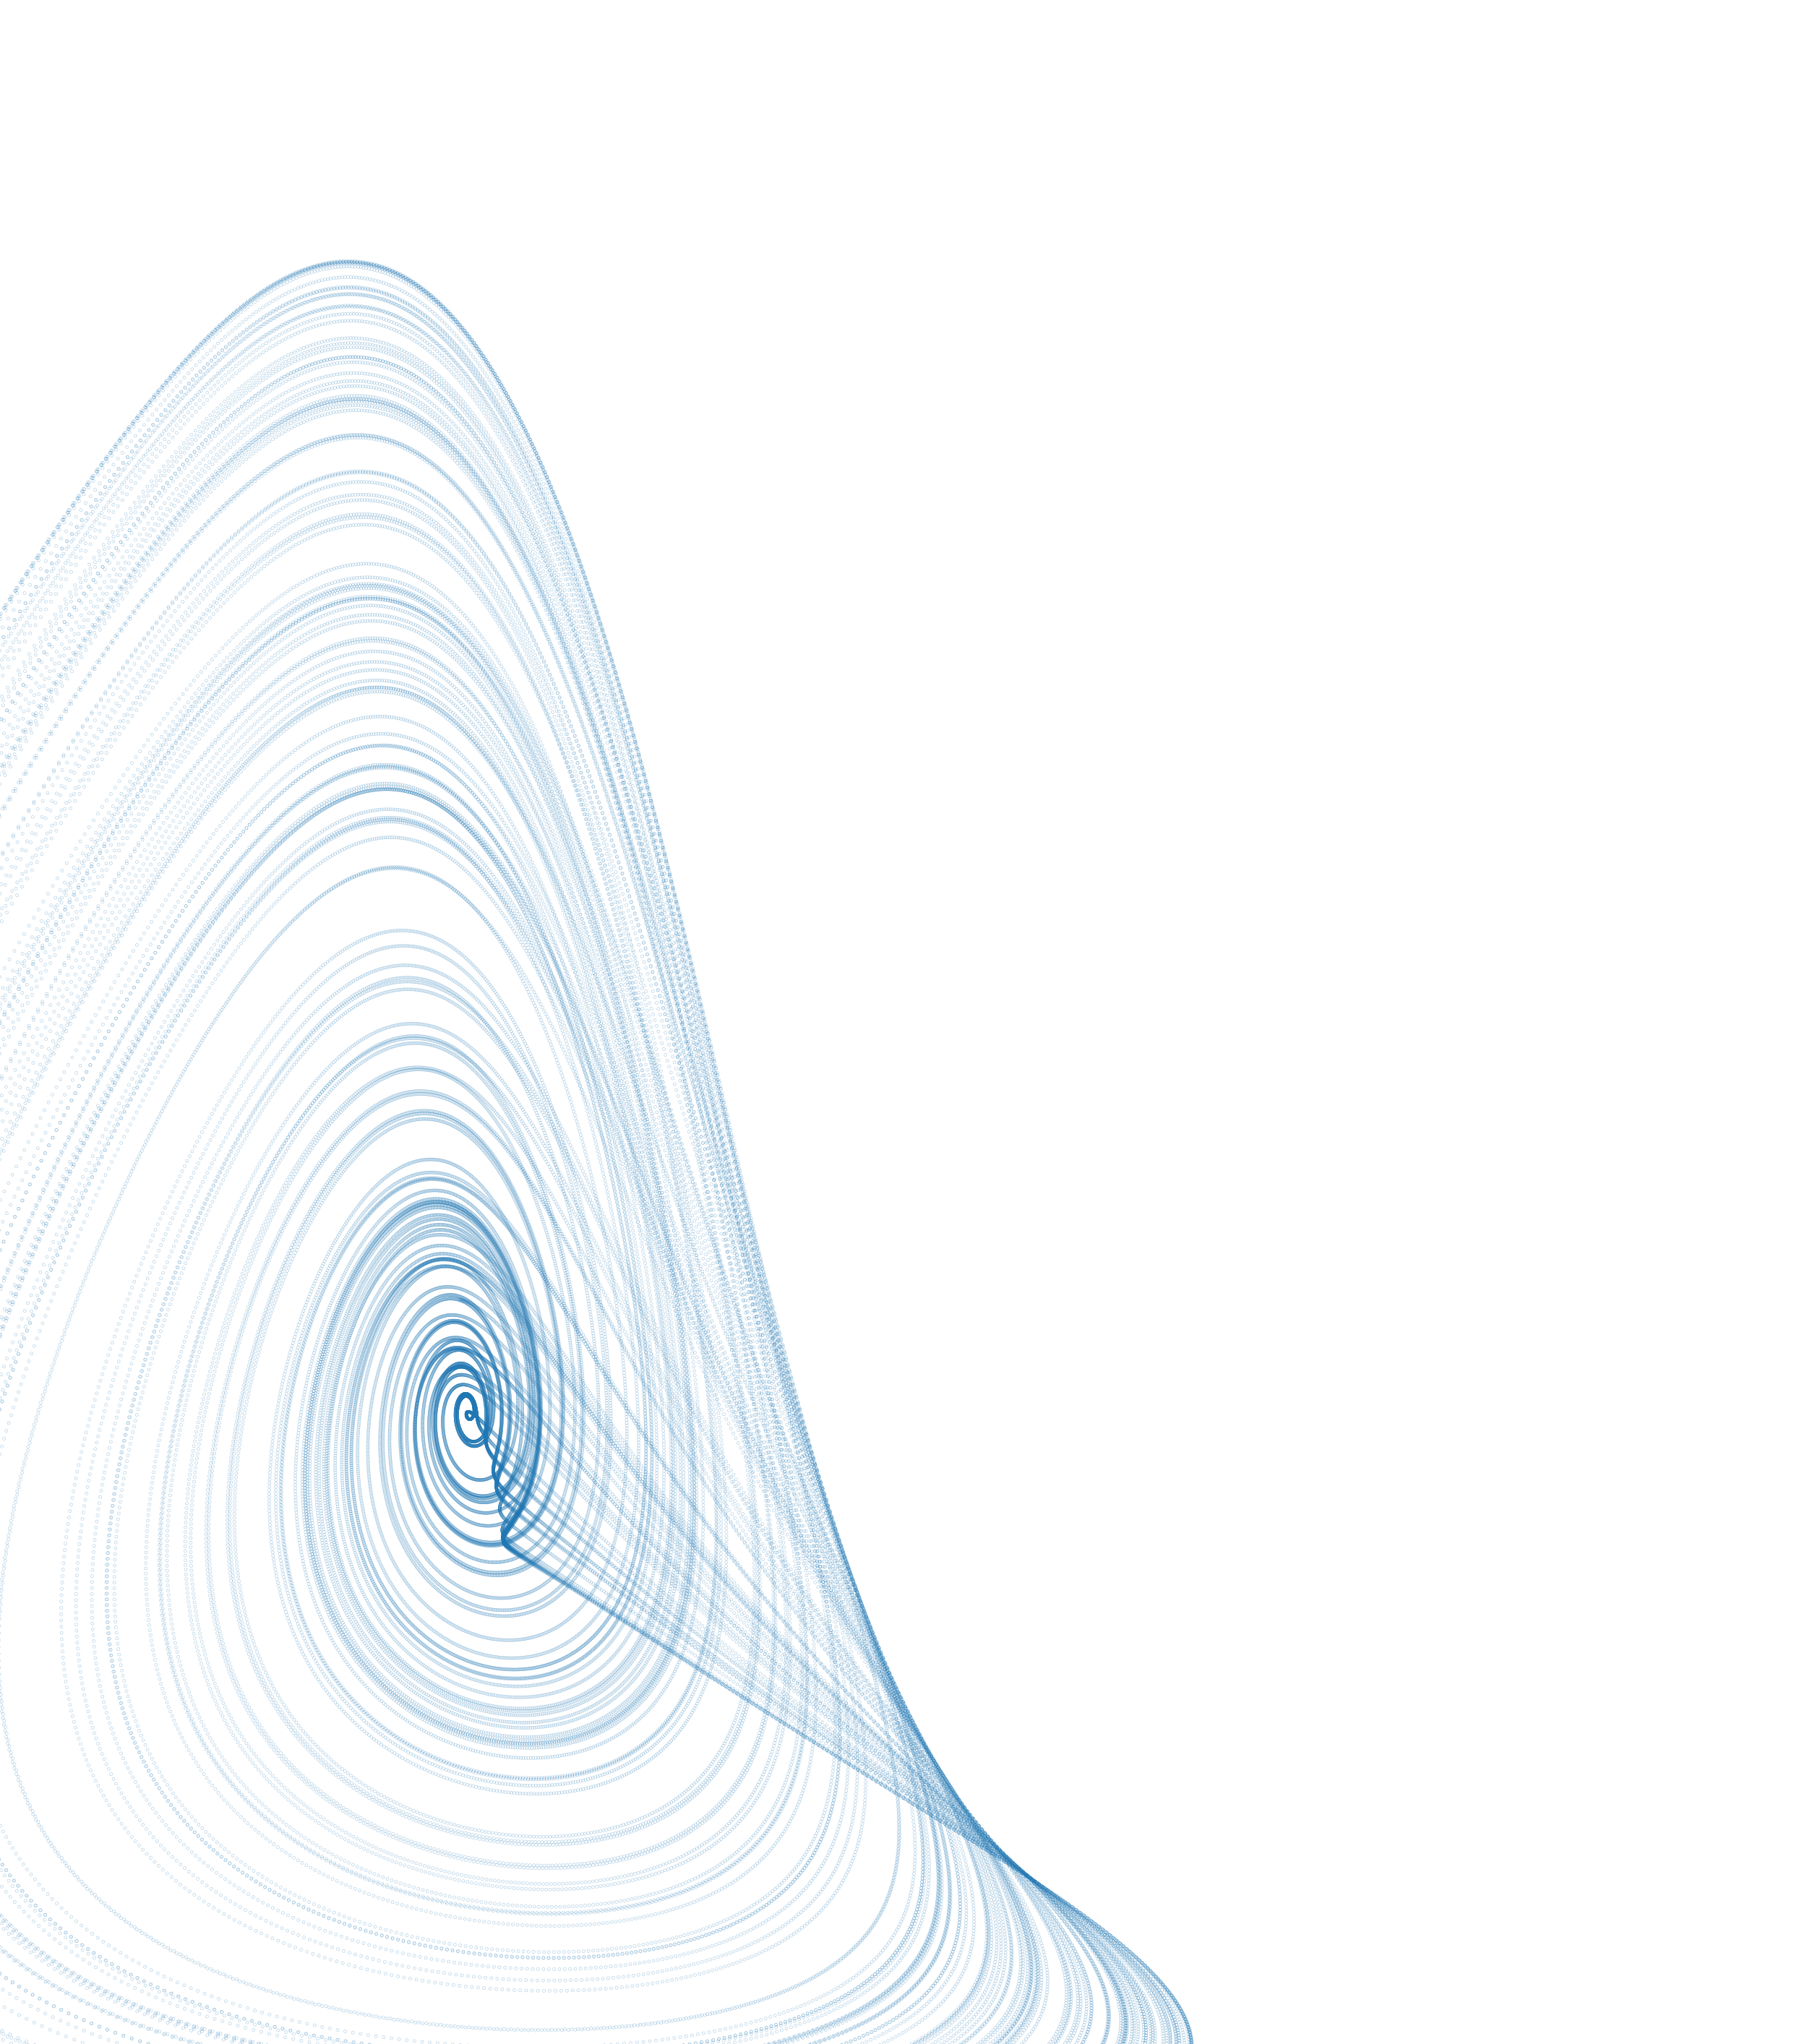
\includegraphics[height=1.1\paperheight,width=1.1\paperwidth]{./figures/LV_copertina_crop.png}};
    \end{tikzpicture}}
\begin{frame} %%  Titolo  %%
   \titlepage  
\end{frame}}  %%%%%%%%%%%%%%

\section{Introduzione} %%%%%%%%%%%%%  Frames  %%%%%%%%%%%%%
%%%%%%%%%%%%%
%  Frame 1  %
%%%%%%%%%%%%%
\begin{frame}
\frametitle{Equazioni Differenziali per Specie in Competizione}
\framesubtitle{Modello Generale}
\begin{itemize}
    \item $x_i$: popolazione della $i$-esima specie.
    \item Spazio degli stati:
	\[
	    R_+^n = \left\{\v{x}\in \mathbb{R}^n \ | \ \v{x}= \left(x_1, x_2, \ldots, x_n\right), \ x_i \ge 0\right\}
	\] 
    \item Dinamica delle popolazioni:
	\begin{equation}
	    \frac{\text{d} x_i}{\text{d} t} = x_i M_i(\v{x}), \qquad i = 1, \ldots, n
	\end{equation}
\end{itemize}
\end{frame}

%%%%%%%%%%%%%
%  Frame 2  %
%%%%%%%%%%%%%
\begin{frame}
\frametitle{Equazioni Differenziali per Specie in Competizione}
\framesubtitle{Condizioni su $M_i$}
\[
    \frac{\text{d} x_i}{\text{d} t} = x_i M_i(\v{x}), \qquad i = 1, \ldots, n
.\] 
\begin{enumerate}
    \item Funzione liscia: $M_i: \mathbb{R}_+^n \to \mathbb{R}$,  $M_i \in C^{\infty}$.
	\label{en:c1}
    \item Affollamento inibisce la crescita: $\forall \ i, j \in \left[1, \ldots n\right] \times \left[1, \ldots n\right]$ 
	\label{en:c2}
	\[
	    \text{Se } x_i > 0  \implies \frac{\partial M_i}{\partial x_j} < 0
	\] 
    \item Risorse limitate: $\exists \ K\in \mathbb{R}$, $K>0$:
	\[
	    \forall i \text{ se } \left|\v{x}\right| > K \implies  M_i(\v{x})  < 0
	\] 
	\label{en:c3}
\end{enumerate}
\end{frame}

%%%%%%%%%%%%%
%  Frame 3  %
%%%%%%%%%%%%%
\begin{frame}
\frametitle{Equazioni Differenziali per Specie in Competizione}
\framesubtitle{Modello di partenza}
\[
M_i(\v{x}) = 1-\sum_{j=1}^{n} x_j
.\] 
Bordo invariante:
\[
    \partial \mathbb{R}^n_+ \equiv \left\{\v{x}\in \mathbb{R}^n_+ \ | \ \text{ qualche } x_i = 0\right\}
.\] 
Se $t\to \infty$ le soluzioni finiscono nell'insieme invariante:
\[
    \Delta_1 \equiv \left\{\v{x}\in \mathbb{R}^n_+ \ | \ \sum_{i}^{n} x_i = 1\right\}
.\] 
Dimostrazione:
\[
    \sum_{i}^{n} x_i = y \implies  \frac{\text{d} y}{\text{d} t} = y(1-y) \implies  
    \begin{cases}
        y=0 \text{ instabile}\\
        y=1 \text{ stabile}
    \end{cases}
\] 
\end{frame}

%%%%%%%%%%%%%
%  Frame 4  %
%%%%%%%%%%%%%
\begin{frame}
\frametitle{Equazioni Differenziali per Specie in Competizione}
\framesubtitle{Prima generalizzazione del modello: definizioni}
\begin{itemize}
    \item $\Delta_0 \equiv \left\{\v{x}\in \mathbb{R}^n_+ \ | \ \sum_{i}^{\infty} x_i = 0\right\}$
    \item $\beta : \mathbb{R}\to \mathbb{R}, \beta(t) \in C^{\infty}$,
	    $\beta (t) = 
            \begin{cases}
	    1 \text{ se } t \in U_{\delta}(1), \delta<\frac{1}{2} \\
		0 \text{ se } \left|t + 1\right| > \frac{1}{2}
            \end{cases}$
    \item $h: \mathbb{R}^n_+ \to \Delta_0$:
	\[
	    h(\v{x}) = \left(\frac{1}{n}\right)I_0- \frac{\v{x}}{\sum_{i}^{n} x_i}; \qquad
	    I_0 \equiv \left(1, 1, \ldots, 1\right) \in \mathbb{R}^n_+
	.\] 
    \item $m_i:\mathbb{R}^n_+ \to \Delta_0$:
	\[
	     m_i(\v{x}) = \frac{1}{x_i}\beta\left(\sum_{j}^{n} x_j\right) \left(\prod_{j=1}^{n} x_j \right)h(\v{x}); \qquad \sum m_i x_i = 0
	.\] 
\end{itemize}
\end{frame}

%%%%%%%%%%%%%
%  Frame 4  %
%%%%%%%%%%%%%
\begin{frame}
\frametitle{Equazioni Differenziali per Specie in Competizione}
\framesubtitle{Prima generalizzazione del modello: l'evoluzione segue $h(\v{x})$}
\begin{equation}
    \frac{\text{d} x_i}{\text{d} t} = x_i\left(M_i + \eta m_i\right) \equiv x_i N_i; \qquad  \eta > 0
    \label{eq:smale2}
\end{equation}
\[
    N_i: \mathbb{R}^n_+ \to \mathbb{R}, \quad N_i \in C^{\infty}
.\] 
\begin{itemize}
    \item Preso $\eta$ sufficientemente piccolo $N_i$ soddisfa \ref{en:c2} e \ref{en:c3}.
    \item L'insieme $\Delta_1$ è ancora un attracting set poiché $\sum_{i}^{n} m_ix_i = 0$. 
\end{itemize}
Dinamica su $\Delta_1$:
\[
    \frac{\text{d} \v{x}}{\text{d} t} = \eta  \v{x} m \propto h(\v{x})  = \frac{1}{n}I_0 - \frac{\v{x}}{1}
.\] 
Un unico punto stazionario in $\v{x} = \frac{1}{n}I_0 \in \mathbb{R}^n_+$ (per soluzioni che non stanno su $\partial \mathbb{R}^n_+$).
\end{frame}

%%%%%%%%%%%%%
%  Frame 5  %
%%%%%%%%%%%%%
\begin{frame}
\frametitle{Equazioni Differenziali per Specie in Competizione}
\framesubtitle{Seconda generalizzazione del modello}
\[
    \frac{\text{d} x_i}{\text{d} t} = x_i\left(M_i + \eta m_i\right) \equiv x_i N_i; \qquad  \eta > 0
.\] 
Siano due funzionali:
\begin{itemize}
    \item $h_0: \Delta_1 \to \Delta_0$, $h_0 \in C^{\infty}$.
    \item $h:\mathbb{R}^n_+ \to \Delta_0$, $h\in C^{\infty}$.
\end{itemize}
tali per cui $h_0 = h_1$ in $\Delta_1$. Per $\eta$ sufficientemente piccolo si hanno le condizioni \ref{en:c1}, \ref{en:c2}, \ref{en:c3}.\\
Prese delle soluzioni non appartenenti a $\partial \mathbb{R}^n_+$ la dinamica asintotica sull'attracting set $\Delta_1$ sarà descritta da:
\[
    \frac{\text{d} \v{x}}{\text{d} t} = h_0(\v{x}) 
.\] 
\end{frame}

%%%%%%%%%%%%%
%  Frame 7  %
%%%%%%%%%%%%%
\begin{frame}
\frametitle{Equazioni Differenziali per Specie in Competizione}
\framesubtitle{Tipo di soluzioni al variare della dimensione}
\begin{itemize}
    \item $n=2$:\\
	$\Delta_1$ ha dimensione 1, le soluzioni in $\Delta_1$ tenderanno ad un punto stazionario stabile (strutturalmente stabile).
    \item $n = 3$:\\
	$\Delta_1$ ha dimensione 2, possiamo sceglierlo in modo tale che presenti un ciclo limite $\gamma$ (strutturalmente stabile).
    \item $n\ge 5$:\\
	$\Delta_1$ è almeno di dimensione 4, le soluzioni in $\Delta_1$ non è detto siano strutturalmente stabili.
\end{itemize}
\end{frame}

%%%%%%%%%%%%%
%  Frame 8  %
%%%%%%%%%%%%%
\begin{frame}
\frametitle{Il Sistema di Lotka Volterra Competitivo}
$n$ specie $x_i$ ($i = 1, \ldots, n$) che competono per le risorse.
\begin{equation}
    \frac{\text{d} x_i}{\text{d} t} = r_i x_i \left(1-\sum_{j}^{n} a_{ij}x_j\right)
    \label{eq:LVC}
\end{equation}
\begin{itemize}
    \item $r_i$: Rate di crescita di $x_i$.
    \item $a_{ij}$: Parametro di competizione tra $x_i$ e $x_j$.
\end{itemize}
\vspace{1.5em}
\begin{equation}
    r_i > 0 \qquad  a_{ij} \ge 0
    \label{eq:cond_ar}
\end{equation}
\[
    r_0 =  a_{ii} = 1
.\] 
\end{frame}


\section{Studio della stabilità}%
\input{Slides/2_Stabilità.tex}
\section{Ricerca del caos}%
%%%%%%%%%%%%%
%  Frame 1  %
%%%%%%%%%%%%%
\begin{frame}
\frametitle{Caos in Dimensione 3}
\framesubtitle{Teorema di Shil'nikov}
A. Arneodo et al. dimostrano che rilassando la \ref{en:c2}) si può ottenere un attrattore strano con $n=3$.\\
Rilassare la 2) significa poter scegliere $a_{ij} < 0$.
\begin{block}{Teorema di Shil'nikov}
Se il sistema linearizzato in $\v{x}^*_s$ è della forma (Saddle-Focus):
\[
    \begin{cases}
	\dot{x} = \left(\rho  + i\omega\right) x \\
	\dot{y} = \left(\rho  - i\omega\right) y \\
	\dot{z} = \lambda z
    \end{cases} 
    \qquad \lambda > -\rho > 0
\] 
ed $\exists$ curva $\Gamma_0$ che lascia $\v{x}^*_s$ e vi ritorna per $t\to \infty$ allora ogni intorno di $\Gamma_0$ contiene un insieme numerabile di orbite periodiche instabili (di tipo sella).
\end{block}
\end{frame}

%%%%%%%%%%%%%
%  Frame 2  %
%%%%%%%%%%%%%
\begin{frame}
\frametitle{Caos in Dimensione 3}
\framesubtitle{Metodo Euristico di costruzione dell'attrattore}
\[
    r_i = 1 \qquad \frac{\text{d} x_i}{\text{d} t} = x_i \sum_{j=1}^{3} a_{ij}(1-x_j) 
.\] 
\begin{itemize}
    \item Si fissano casualmente 8 di 9 parametri di $a_{ij}$:
	\[
	    a_{ij} =\begin{pmatrix}
	        0.5 & 0.5 & 0.1 \\
	        -0.5 & -0.1 & 0.1 \\
	        \mu & 0.1 & 0.1 \\
	    \end{pmatrix}
	\] 
    \item $\mu$ si fissa in modo da avere
	\begin{itemize}
	    \item $\mu  > \mu_0$ $\implies$ Uno dei punti $Q_{ij}\equiv A$ di tipo "Saddle-Focus".
	    \item $\mu > \mu_H > \mu_0$ $\implies$ Il punto $B$: $x_i=1$ $\forall i = 1, 2, 3$ con biforcazione di Hopf.
	\end{itemize}
    \item Si fa variare $\mu$ al di sopra della biforcazione.
\end{itemize}
\end{frame}

%%%%%%%%%%%%%
%  Frame 3  %
%%%%%%%%%%%%%
\begin{frame}
\frametitle{Caos in Dimensione 3}
\framesubtitle{Formazione dell'orbita omoclinica}
\begin{figure}[H]
    \centering
    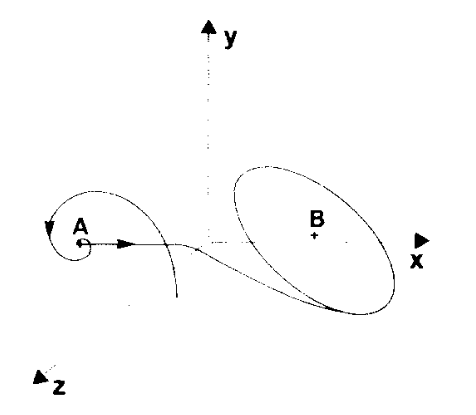
\includegraphics[width=0.4\textwidth]{figures/omo1.png}
    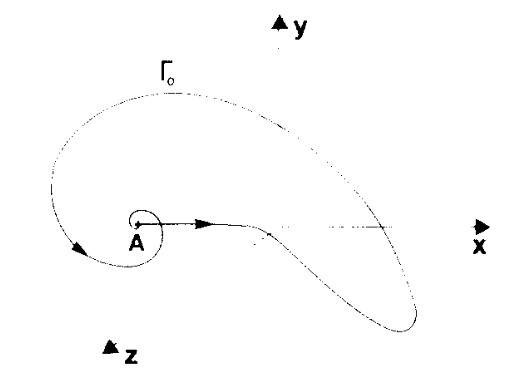
\includegraphics[width=0.4\textwidth]{figures/omo2.png}
    \caption{Costruzione grafica della curva $\Gamma_0$ del teorema di Shil'nikov (Arneodo et al). }
    \label{fig:figures-omo2-png}
\end{figure}
\begin{center}
Simulazione del sistema al variare di $\mu$ \textcolor{blue}{\href{run:link/Animated_trans.html}{(trans)}}, \textcolor{blue}{\href{run:link/Animated_no_trans.html}{(no trans)}}
\end{center}
\end{frame}

%%%%%%%%%%%%%
%  Frame 4  %
%%%%%%%%%%%%%
\begin{frame}
\frametitle{Caos in Dimensione 3}
\framesubtitle{Costruzione dell'attratore}
\begin{figure}[H]
    \centering
    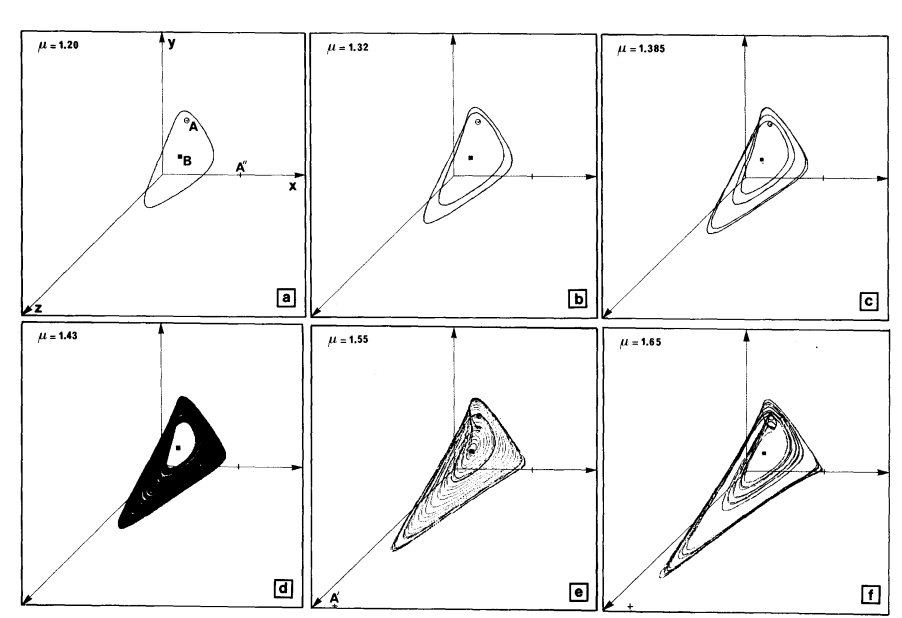
\includegraphics[width=0.8\textwidth]{figures/Hopf.png}
    \caption{Formazione dell'attrattore strano a partire dal sistema della slide precedente (Arneodo et al.)}
    \label{fig:figures-Hopf-png}
\end{figure}
\end{frame}

%%%%%%%%%%%%%
%  Frame 4  %
%%%%%%%%%%%%%
\begin{frame}
\frametitle{Caos in dimensione 4}
\framesubtitle{Estensione dei parametri ottenuti in dimensione 3}
\begin{block}{Coste et al.:}
Ogni sistema di LV di dimensione $n+1$ con $r_i = r_j$ $i, j = 1, \ldots, n+1$ può essere ridotto ad un sistema di LV di dimensione $n$ e viceversa.
\end{block}
\vspace{1em}
$\implies$ è possibile ottenere caos in dimensione 4 rispettando anche le richieste \ref{en:c1}), \ref{en:c2}), \ref{en:c3}).
\end{frame}

%%%%%%%%%%%%%
%  Frame 5  %
%%%%%%%%%%%%%
\begin{frame}
\frametitle{Caos in dimensione 4}
\framesubtitle{Generalizzare i risultati di Arneodo et al.}
\begin{block}{Alcuni risultati di Vano et al.}
\begin{itemize}
    \item Generalizzare il modello:
	\begin{itemize}
	    \item $r_i \neq r_j$.
	\end{itemize}
    \item Analisi numerica:
	\begin{itemize}
	    \item Massimizzare l'esponente di Lyapunov positivo.
	    \item Vincolare le popolazioni $x_i \ge x_{\text{lim}}$ (evitare estinzione).
            \item Analisi della rarità delle soluzioni caotiche nello spazio dei parametri.
	\end{itemize}
\end{itemize}
\end{block}
\end{frame}

%%%%%%%%%%%%%
%  Frame 6  %
%%%%%%%%%%%%%
\begin{frame}
\frametitle{Caos in dimensione 4}
\framesubtitle{Analisi numerica}
\begin{itemize}
    \item $r_i$, $a_{ij}$: 20 parametri iniziali.
	\begin{itemize}
	    \item $r_0=1$ 
	    \item $a_{ii} = 1$ 
	\end{itemize}
	Restano 15 parametri liberi.
    \item Ricerca numerica nello spazio dei parametri:
	\begin{itemize}
	    \item Aggiornare i parametri.
	    \item Simulare il sistema.
	    \item Fermare la simulazione se $x_i < x_{\text{lim}}$ (e tornare in cima).
	    \item Calcolare gli esponenti di Lyapunov.
	    \item Salvare la configurazione $\overline{r}_i, \overline{a}_{ij}$ che massimizza gli esponenti.
	\end{itemize}
\end{itemize}
\end{frame}

%%%%%%%%%%%%%
%  Frame 7  %
%%%%%%%%%%%%%
\begin{frame}
\frametitle{Caos in dimensione 4}
\framesubtitle{Risultati ottenuti}
\[
    r =\begin{bmatrix}
        1 \\
        0.72 \\
        1.53 \\
        1.27 \\
    \end{bmatrix} \qquad 
    a =\begin{bmatrix}
        1 & 1.09 & 1.52 & 0 \\
        0 & 1 & 0.44 & 1.36 \\
        2.33 & 0 & 1 & 0.47 \\
        1.21 & 0.51 & 0.35 & 1 \\
    \end{bmatrix}
\] 
\vspace{1em}
\[
    LEs = \left[0.0203, 0, -0.2748, -1.0289\right]; \qquad  \sum_{}^{} LEs = -1.2834
.\] 
\vspace{0.5em}
\[
    D_{KY} = 2.074
.\] 
\vspace{0.5em}
\begin{center}
\textcolor{blue}{\href{run:link/LV_simu.html}{Simulazione del sistema\ldots}}
\end{center}
\begin{center}
\textcolor{blue}{\href{run:link/Max_LE.html}{Distribuzione degli esponenti di Lyapunov}}
\end{center}
\end{frame}

%%%%%%%%%%%%%
%  Frame 8  %
%%%%%%%%%%%%%
\begin{frame}
\frametitle{Ottenere il Grafico di Biforcazione}
Per ottenere il grafico di biforcazione si utilizza un parametro $s$:
\[
    a_{ij} = \begin{cases}
	a_{ij} &\text{ se } i = j\\
	s\cdot a_{ij} & \text{ se } i \neq j
    \end{cases}
.\] 
$\forall s \in S \subset \mathbb{R}$ (intervallo arbitrario):
\begin{itemize}
    \item Si simula il sistema.
    \item Si scartano le prime $n$ iterazioni (termalizzazione).
    \item Si salvano tutti i massimi locali di una delle variabili al variare di $s$. 
\end{itemize}
\end{frame}

%%%%%%%%%%%%%
%  Frame 9  %
%%%%%%%%%%%%%
\begin{frame}
\frametitle{Rarità del Caos e Grafico di Biforcazione}
\begin{figure}[H]
    \centering
    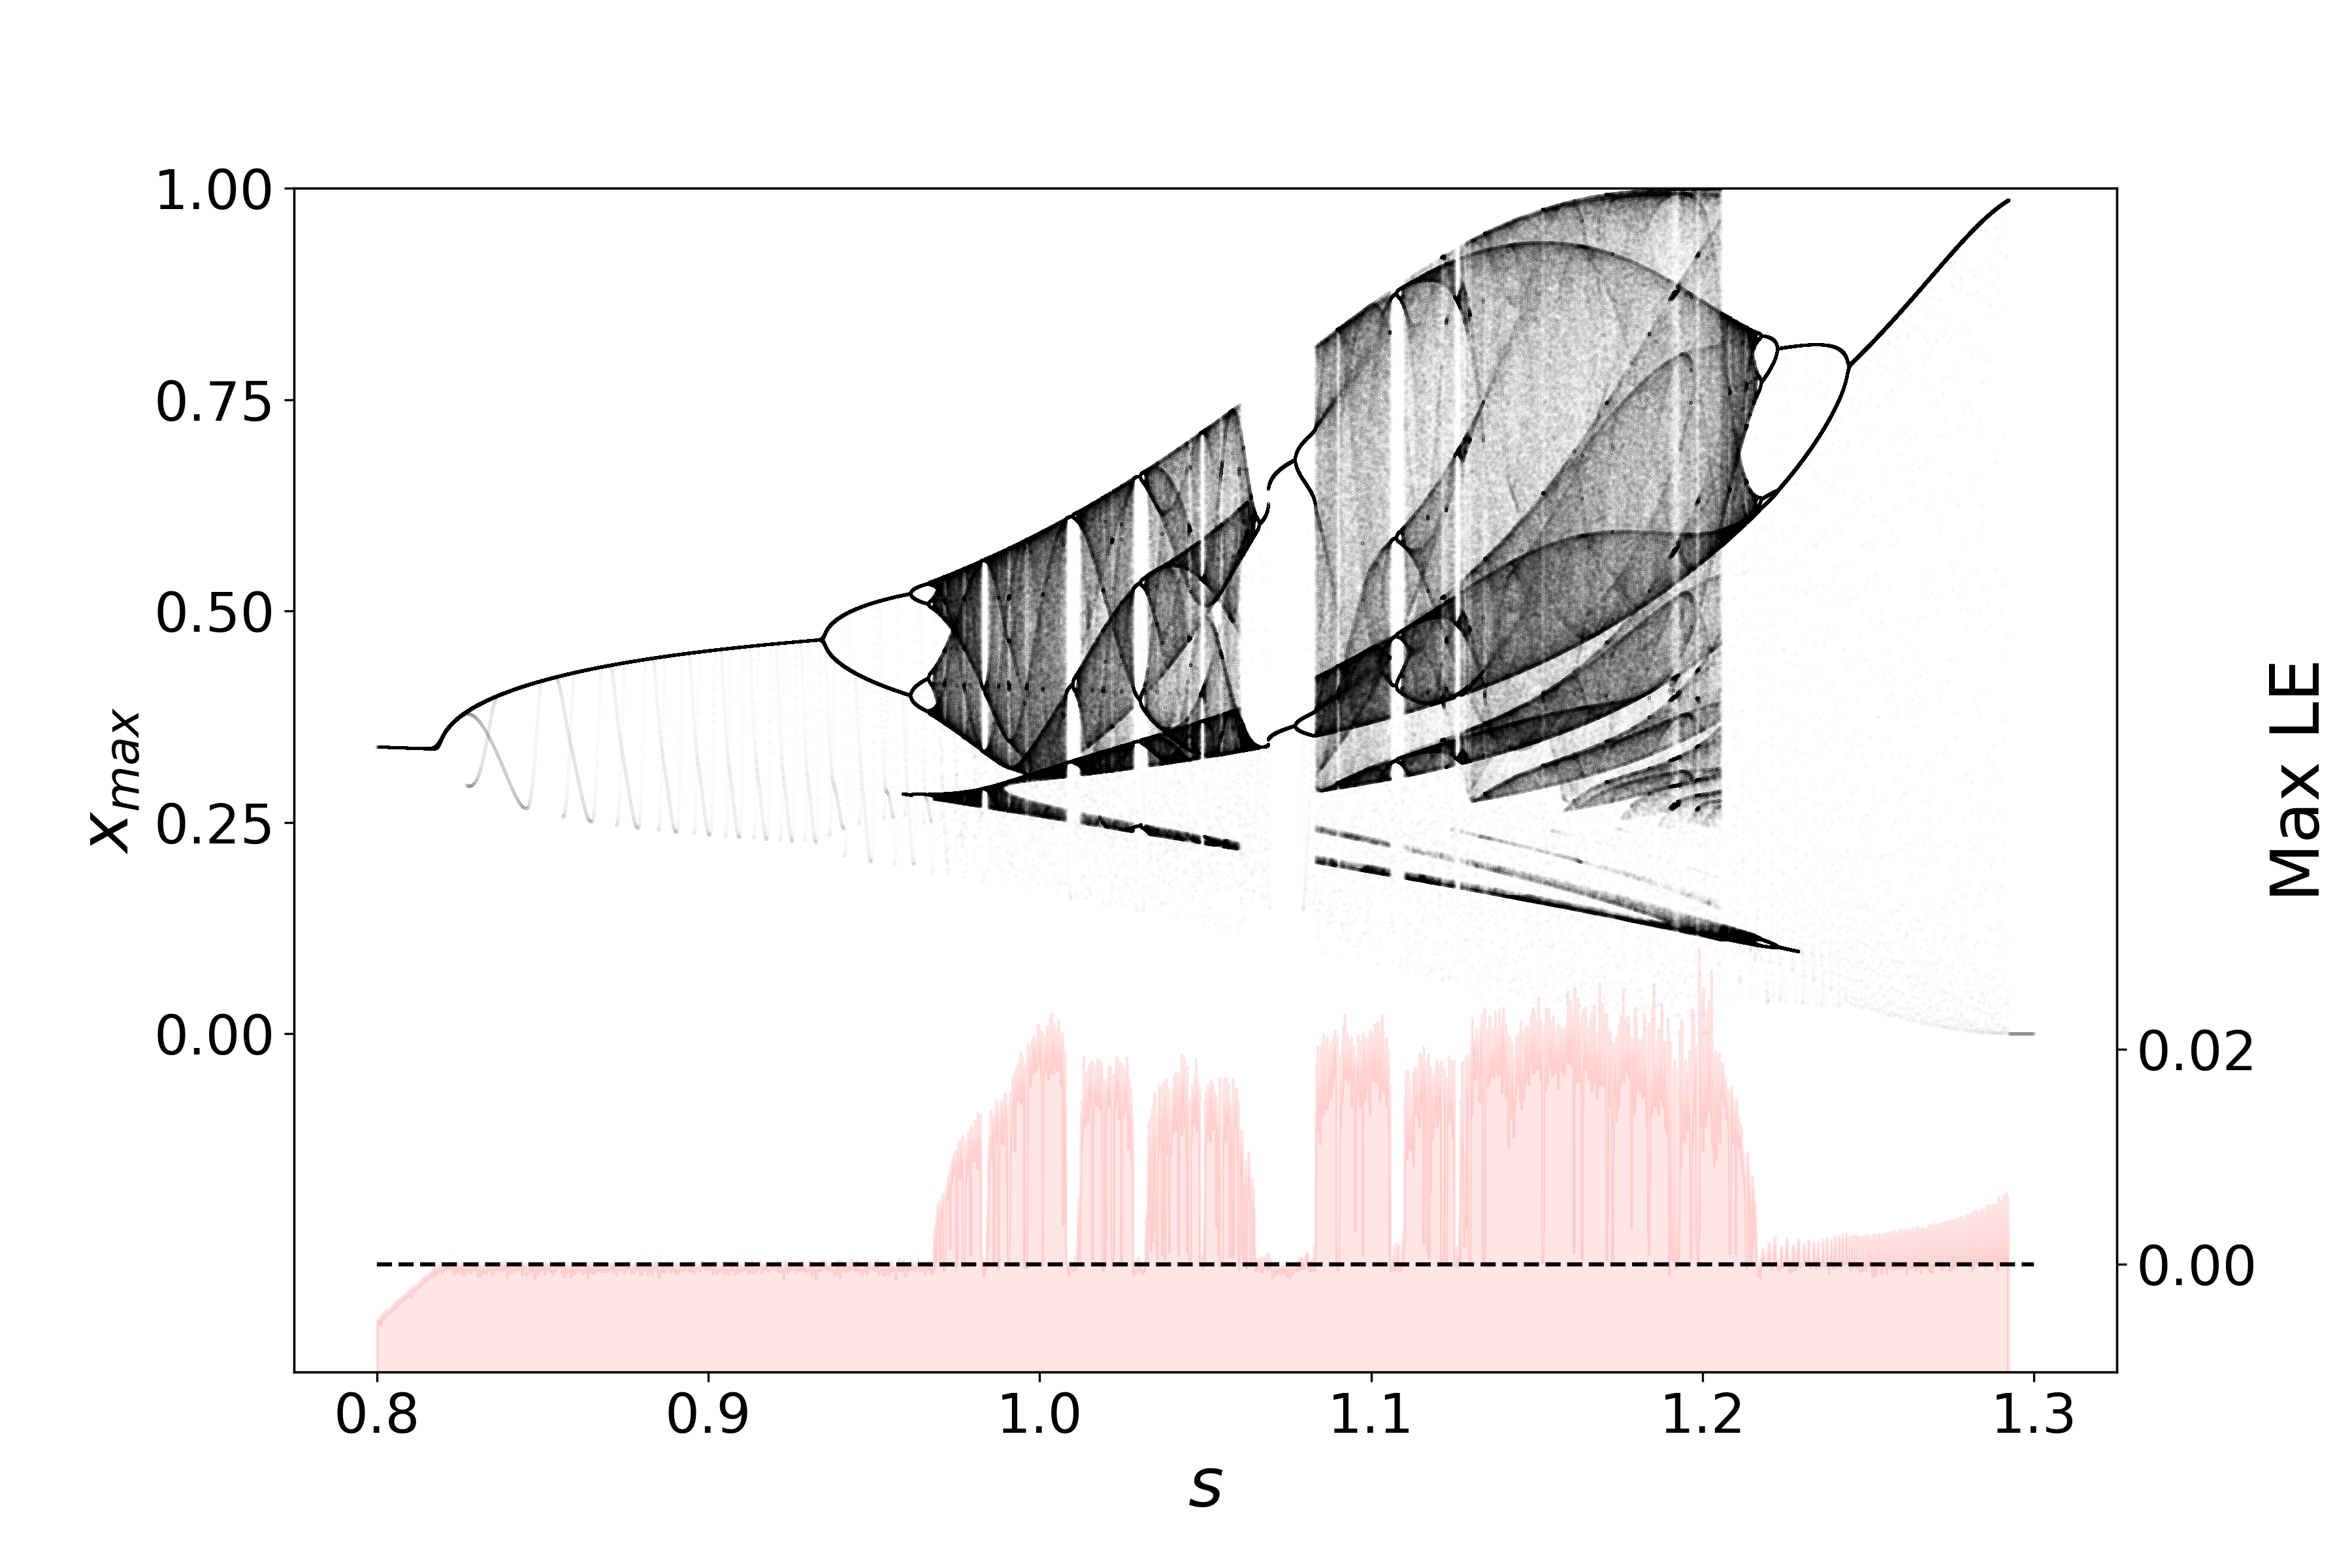
\includegraphics[width=\textwidth]{figures/bif_diag.png}
\end{figure}
\end{frame}

%\section*{Appendice: Esponenti di Lyapunov}%
%%%%%%%%%%%%%%
%  Frame 1  %
%%%%%%%%%%%%%
\begin{frame}
\frametitle{Definizione di Esponenti di Lyapunov}
\begin{itemize}
    \item $\v{x}_0\in \mathbb{R}^n$: Condizione iniziale.
    \item $\v{y}_0\in \mathbb{R}^n$ Perturbazione.
    \item $\varphi_t$ Flusso di fase.
    \item $U_0$ "Parallelepipedo" con vertici $\v{y}_i$, $i = 1, \ldots , p$.
\end{itemize}
\begin{block}{LE di ordine 1}
\[
    \lambda (\v{x}_0, \v{y}_0) = \lim_{t \to \infty} \frac{1}{t}\ln\left|\left|D_{\v{x}_0}\varphi_t(\v{x}_0) \v{y}_0\right|\right|
.\] 
\end{block}
\begin{block}{LE di ordine $p\le n$}
\[
    \lambda^p(\v{x}_0, U_0) = \lim_{t \to \infty} \frac{1}{t}\ln\left[\text{Vol}^p\left(D_{\v{x}_0}\varphi_t(U_0)\right)\right]
.\]
\end{block}
\end{frame}

%%%%%%%%%%%%%
%  Frame 2  %
%%%%%%%%%%%%%
\begin{frame}
\frametitle{Proprietà degli Esponenti di Lyapunov e dinamica tangente}
\begin{block}{Equazione Variazionale}
Andamento delle possibili perturbazioni:
\[
    \dot{\Phi}_t (\v{x}_0)  = D_{\v{x}}F\left(\varphi_t(\v{x}_0) \right)\cdot \Phi_t(\v{x}_0) \qquad  \Phi_0(\v{x}_0) = \mathbb{I}
.\] 
\end{block}
\begin{block}{Teorema di Oseledec}
Prese $\v{y}_i$, $i=1, \ldots, p$, perturbazioni linearmente indipendenti:
\begin{equation}
    \lambda^p(\v{x}_0, U_0)  = \lambda(\v{x}_0, \v{y}_1)  + \ldots + \lambda(\v{x}_0, \v{y}_p) 
    \label{eq:sumlambda}
\end{equation}
\end{block}
\begin{block}{Spettro di Lyapunov}
    L'insieme dei $\lambda (\v{x}_0, \v{y}_i)$ con $\v{y}_i$, $i = 1, \ldots, n$ perturbazioni linearmente indipendenti è chiamato spettro di Lyapunov.
\end{block}
\end{frame}

%%%%%%%%%%%%%
%  Frame 3  %
%%%%%%%%%%%%%
\begin{frame}
\frametitle{Calcolo dello spettro di Lyapunov (Benedettin)}
\framesubtitle{Utilizzo dell'algoritmo di Gran-Schmidt}
Dato un set $\left\{\v{y}_1, \ldots, \v{y}_p\right\}$  linearmente indipendenti ortonormalizziamo con Gran-Schmidt:
\[\begin{aligned}
    & \v{w}_1 = \v{y}_1 &\quad&\quad& \v{v}_1 = \frac{\v{w}_1}{\left|\left|\v{w}_1\right|\right|}\\
    & \v{w}_p = \v{y}_p - \sum_{i = 1}^{p-1} \left<\v{y}_p, \v{v}_i\right>\v{v}_i &\quad&\quad& \v{v}_p =\frac{\v{w}_p}{\left|\left|\v{w}_p\right|\right|} 
.\end{aligned}\]
Il volume del parallelepipedo $U_0$ è quindi:
\[
    \text{Vol}\left\{\v{y}_1, \ldots, \v{y}_p\right\} = \left|\left|\v{w}_1\right|\right|\cdot \cdot \cdot \left|\left|\v{w}_p\right|\right|
.\] 
\end{frame}


%%%%%%%%%%%%%
%  Frame 4  %
%%%%%%%%%%%%%
\begin{frame}
\frametitle{Calcolo degli esponenti di Lyapunov (Benedettin)}
\framesubtitle{Idea algoritmica}
\begin{itemize}
    \item Scelta perturbazione iniziale $U_0 = \left[\v{y}^0_1, \ldots, \v{y}^0_n\right]$, $\v{y}_i \in \mathbb{R}^n$ ed intervallo di integrazione $T$.
    \item Evoluzione della mappa tangente:
	\[
	    U_1 = D_{\v{x}_0}\varphi_T(U_0) = J_T(\v{x}_0) \left[\v{y}^0_1,\ldots, \v{y}^0_n\right]
	.\] 
    \item Ortogonalizzo $U_1$, ottengo vettori ortogonali $\v{w}^1_i$ e ortonormali $V_1 \equiv \left[\v{v}^1_1, \ldots, \v{v}^1_n\right]$. 
    \item Il volume aumenta di un fattore $\left|\left|\v{w}^1_1\right|\right|\cdot \cdot \cdot \left|\left|\v{w}_n^1\right|\right|$ 
	\[
	    \text{Vol}_1^p = \left|\left|\v{w}^0_1\right|\right|\cdot \cdot \cdot \left|\left|\v{w}_n^0\right|\right|\cdot
	    \left|\left|\v{w}^1_1\right|\right|\cdot \cdot \cdot \left|\left|\v{w}_n^1\right|\right|
	.\] 
\end{itemize}
\end{frame}

\begin{frame}
\frametitle{Calcolo degli esponenti di Lyapunov (Benedettin) }
Sostituendo il volume nella definizione ed iterando infinite volte:
\[
    \lambda^n(\v{x}_0, U_0) = \lim_{k \to \infty} \frac{1}{kT}\sum_{i = 1}^{k} 
    \ln\left(\left|\left|\v{w}^i_1\right|\right|\cdot \cdot \cdot \left|\left|\v{w}_n^i\right|\right|\right)
.\] 
Sottraendo $\lambda^{n-1}$ ed usando la \ref{eq:sumlambda}:
\[
    \lambda_n = \lim_{k \to \infty} \frac{1}{kT}\sum_{i = 1}^{k} \ln\left(\left|\left|\v{w}_n^i\right|\right|\right)
.\] 
Si può troncare l'ultima espressione per ottenere $\lambda_1, \ldots, \lambda_n$ 
\end{frame}

\section{Bibliografia}%
\begin{frame}
\frametitle{Bibliografia}
\begin{thebibliography}{9}
    \bibitem{NumLyap} 
    Marco Sandri: \textit{Numerical calculation of Lyapunov exponents}. \\
    Università di Verona (1996)

    \bibitem{MainArt} 
    J. A. Vano et al: \textit{Chaos in low-dimensional Lotka–Volterra models of competition}.\\
    London Mathematical Society (2006)\\ 

    \bibitem{Smale} 
    S. Smale: \textit{On the Differential Equations Of Species in Competition}.\\
    Berkely, California (1976) 

\end{thebibliography}
\end{frame}

\end{document} %%%%%%%%%%%%%%%%%%%%%%%%%%%%%%%%%%%%%%%%
